\section{Qafny: A High-level Quantum Language Admitting a Proof System}
\label{sec:qafny}

\begin{figure}[t]
{\small
\[\hspace*{-0.5em}
\begin{array}{r l l}
\textcolor{blue}{1}
&
\{A(x) * A(y) \}
\;\;\text{where}\;\;
A(\beta) = \beta[0..n] \mapsto \ket{\overline{0}} 
&
\{x[0..n]: \tnort, y[0..n]: \tnort\}
\\[0.2em]
\textcolor{blue}{2}
& \ssassign{x}{}{\ihadh};\\[0.2em]

\textcolor{blue}{3}
&
\textcolor{teal}{
\{x[0..n] \mapsto \dabs{\ihadh}(\ket{\overline{0}}) * A(y) \}
}
&
\textcolor{teal}{
\{x[0..n]: \thadt, y[0..n]: \tnort\}
}
\\[0.2em]
\textcolor{blue}{4}
&
\textcolor{teal}{
\Rightarrow
\{x[0..n] \mapsto C * A(y) \}
}
\;\;\text{where}\;\;
\textcolor{teal}{
C = \shad{2^n}{n}{}
}
&
\textcolor{teal}{
\{x[0..n]: \thadt, y[0..n]: \tnort\}
}
\\[0.2em]
\textcolor{blue}{5}
& \ssassign{y}{}{y\splus 1};
\\[0.2em]

\textcolor{blue}{6}
&
\textcolor{teal}{
\{x[0..n] \mapsto C * y[0..n] \mapsto \dabs{y\splus 1}(\ket{\overline{0}}) \}
}
&
\textcolor{teal}{
\{x[0..n]: \thadt, y[0..n]: \tnort\}
}
\\[0.2em]
\textcolor{blue}{7}
&
\textcolor{teal}{
\Rightarrow
\{x[0..n] \mapsto C * y[0..n] \mapsto \ket{\overline{0}}\ket{1} \}
}
&
\textcolor{teal}{
\{x[0..n]: \thadt, y[0..n]: \tnort\}
}
\\[0.2em]
\textcolor{blue}{8}
& 
\textcolor{teal}{
\Rightarrow
\{ E(0) \}
}
\;\;
\texttt{where}\;\;
\textcolor{teal}{E(t) =}
&
\textcolor{teal}{
\{x[0..n]: \thadt, \{x[0..0],y[0..n]\}: \tcht\}
}
\\
&
\qquad\qquad\quad\;
\textcolor{teal}{
\begin{array}{l}
x[t..n] \mapsto \shadi{2^{n \,\sminus\,  t}}{n \,\sminus\, t}{}\;*
\\
\{x[0..t],y[0..n]\} \mapsto \schai{2^t}{\frac{1}{\sqrt{2^t}}}{i}{\ket{a^{i}\;\%\;N}}
\end{array}
}
\\[0.2em]
\textcolor{blue}{9}
&\sqforh{\sint{j}{0}}{j\,\slt\, n}{x[j]}{\dplus{j}}
\\[0.2em]
\textcolor{blue}{10}
&
\quad\{E(j) \}
&
\{x[j..n]: \thadt, \{x[0..j],y[0..n]\}: \tcht\}
\\[0.2em]
\textcolor{blue}{11}
&
\quad\ssassign{y}{}{a^{2^j}y\;\%\; N};
\\[0.2em]
\textcolor{blue}{12}
&
\textcolor{teal}{
\{E(n) \}
}
&
\textcolor{teal}{
\{x[0..0]: \thadt, \{x[0..n],y[0..n]\}: \tcht\}
}
\\[0.2em]
\textcolor{blue}{13}
&
\textcolor{teal}{
\Rightarrow
\{\{x[0..n],y[0..n]\} \mapsto \schai{2^{n}}{\frac{1}{\sqrt{2^{n}}}}{i}{\ket{a^{i}\;\%\;N}} \}
}
&
\textcolor{teal}{
\{\{x[0..n],y[0..n]\}: \tcht\}
}
\\[0.2em]
\textcolor{blue}{14}
& \sexp{u}{\smea{y}}{...}
\\[0.2em]
\textcolor{blue}{15}
&
\textcolor{purple}{
\big{\{}
\begin{array}{l}
x[0..n] \mapsto \smch{\frac{1}{\sqrt{s}}}{s}{t\,\splus\,k p} 
\wedge
p = \texttt{ord}(a,N)
\\
\wedge\;
u=(\frac{p}{2^n},a^{t}\;\%\;N)
\wedge
s=\texttt{rnd}(\frac{2^n}{p})
\end{array}
\big{\}}
}
&
\textcolor{purple}{
\{\{x[0..n]\}: \tcht\}
}
\end{array}
\]
}
\caption{Pre-measurement quantum steps of the Shor's algorithm. $\sord{a,N}$ gets the order of $a$ and $N$. $\srnd{r}$ rounds $r$ to the nearest integer. The right-hand-side contains the types for the sessions involved. $\ket{i}$ is an abbreviation of $\ket{\tos{i}}$.
$\tos{i}$ turns a number $i$ to a bitstring. }
\label{fig:shorqafny}
\end{figure}

We designed \qafny, the core language of QNP,
to express quantum programs in terms of
high-level operations that are abstracted away low-level circuit gates.
The operations in \qafny are analogized to classical array 
aggregate operations so that automated verification is feasible.
\qafny's type system tracks the transformation of sessions
with three types representing the sessions' quantum states.
The \qafny proof system captures the analogy of viewing quantum 
operations as classical aggregate operations 
by utilizing the type system to ensure the session state forms.
All of these features are novel to quantum languages and proof systems. 

\begin{wrapfigure}{r}{8.2cm}
  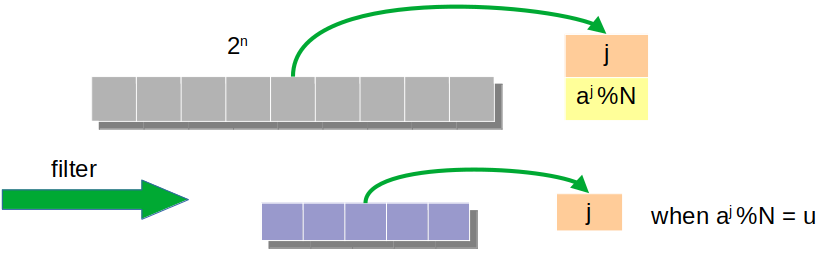
\includegraphics[width=.60\textwidth]{shorsmap}
  \caption{The array analogy of Shor's first half in \Cref{fig:shorqafny}. }
\label{fig:shorsanalog}
\end{wrapfigure}

This section presents \qafny states and the language's syntax, typing, 
semantics, proof system, and soundness/completeness results.  
As a running example, we use the Shor's algorithm~\cite{Shor94} shown in \Cref{fig:shorqafny}. 
Given an integer $N$, Shor's algorithm finds its nontrivial prime factors, which has the following step: (1) randomly pick a number $1 < a < N$ and compute $k=\texttt{gcd}(a,N)$ \footnote{compute the greatest common divisor of $a$ and $N$}; (2) if $k \neq 1$, $k$ is the factor; (3) otherwise, $a$ and $N$ are coprime and we find the order $p$ of $a$ and $N$ \footnote{the order $p$ is the smallest number such that $a^p \% N = 1$}; (4) if $p$ is even and $a^{\frac{p}{2}} \neq -1 \% N$, $\texttt{gcd}(a^{\frac{p}{2}}\pm 1,N)$ are the factors, otherwise, we repeat the process. Step (2) is the Shor's algorithm's quantum component and \Cref{fig:shorqafny} and \Cref{fig:shorqafny2} show its automated proof in QNP. In \Cref{fig:shorexample}, we show the actual implementation and proof in the Qafny tool.

The Shor's pre-measurement quantum steps in \Cref{fig:shorqafny} can be analogized as an efficient array filter operation.
The steps before line 14 (steps at line 2, 5 and 9-11) create a $2^n$-length of pairs, each of which is formed as $(i,a^i \% N)$ where $i\in [0,2^n)$. The measurement in line 14 filters the array as a new one ($x[0..n]$) with all elements $i$ satisfying $a^i \% N=u$ where $u$ is a randomly picked number. Notice that modulo multiplication $f(i)=a^i\%N$ is a periodic function. All elements in $x[0..n]$ satisfy $a^i \% N=u$, which means that 1) there is a smallest $t$ such that $a^t \% N=u$, and 2) all elements can be rewritten as $i=t+kp$ and $p$ is the period of the modulo multiplication function, which is given as the post-condition on the right of line 15.
The implementation and correctness proof in \Cref{fig:shorqafny} exactly reflects the array analogy aspect.
\ignore{
One of the biggest advantage of using \qafny is that we can analogize quantum operations to classical array operations, so that we can utilize the existing automated proof infrastructure in many tools, such as Dafny.
In the Qafny implementation, verifying a quantum program usually requires only the user input of the pre-, post-, and loop invariant. For example, the proof of \Cref{fig:shorqafny} in \qafny requires none of the states marked teal, but only the conditions marked black and purple. \footnote{The purple is also not needed if we combine the Shor's first and second half algorithms together.}
Here, we step by step discuss the states, program syntax, and proofs of the aspect.
}
Notice that only the black and purple parts in \Cref{fig:shorqafny} are required to input in the \qafny implementation, and the teal parts can be inferred by the \qafny proof system. \footnote{The purple is also not needed if we verify the whole Shor's algorithm in \Cref{fig:shorexample}.}

We first introduce \qafny states, syntax, and type system. Then, we discuss its semantics and proof system and metatheories.

\subsection {Classical and Quantum States}

\begin{figure}[t]
{ \small
\[\hspace*{-0.5em}
\begin{array}{l}
\textcolor{blue}{\text{Basic Terms:}}\\[0.2em]
\begin{array}{llcl llcl llcl llcl}
\text{Nat. Num} & m, n & \in & \mathbb{N}
&
      \text{Real} & r & \in & \mathbb{R}
&
      \text{Amplitude} & z & \in & \mathbb{C}
&
\text{Phase} & \alpha(r) & ::= & e^{2\pi i r}

\\
      \text{Variable} & x,y &&

 & \text{Bit} & d & ::= & 0\mid 1       
&
      \text{Bitstring} & c & \in & d^{+}
&
      \text{Basis}& \beta & ::= & (\ket{c})^+
\end{array}
\\[1em]
\textcolor{blue}{\text{Modes, Kinds, Types, and Classical/Quantum Values:}}\\[0.2em]
\begin{array}{llclll} 
      \text{Mode} & g & ::= & \cmode  \mid \mmode\\
      \text{Classical Value} & v & ::= & n \mid (r,n)\\
      \text{Kind} & \overline{g} & ::= & g \mid \qmode{n} \\
      \text{Quantum Type} & \tau & ::= & \tnort &\mid \thadt & \mid \tcht \\
      \text{Quantum Value} & q & ::= & z\beta & \mid \shad{2^n}{n}{\alpha(r_j)} &\mid \ssum{j=0}{m}{z_j\beta_j} \\
    \end{array}
\\[1em]
\textcolor{blue}{\text{Quantum Sessions, Environment, and States}}\\[0.2em]
\begin{array}{llclcl} 
      \text{Range} & re & ::= & x[n..m] \\
      \text{Session} & \kappa & ::= & \overline{re} & \text{concatenated op} & \uplus \\
      \text{Type Environment} & \sigma & ::= & \overline{\kappa : \tau } & \text{concatenated op} & \cup \\
      \text{Quantum State} & \varphi & ::= & \overline{ \kappa : q } & \text{concatenated op} & \cup \\
    \end{array}
\end{array}
  \]
}
  \caption{\qafny element syntax. Each range $x[n..m]$ in a session $l$ represents the number range $[n,m)$ in a qubit array piece $x$. Sessions are finite lists, while type environments and states are finite sets. the operations after "concatenated op" refer to the concatenation operations for session, type environments and quantum states. $(\ket{c})^+$ is a non-empty list of bases $\ket{c_i}$, and refers to $\ket{c_0}...\ket{c_n}=\ket{c_0}\otimes ... \otimes \ket{c_n}=\ket{c_0. ... c_n}$. }
  \label{fig:qafny-state}
\end{figure}

\qafny has three \emph{kinds} of parameters in \Cref{fig:qafny-state}: $\cmode$-kind classical integers \footnote{In the \qafny implementation one can utilize any classical typed parameters in Dafny . For simplicity, we only allow integers in this paper.}, 
$\mmode$-kind classical integers $(r,n)$ with a probability characteristic $r$ representing the theoretical probability of the measurement resulting in the natural number $n$, and $\qmode{n}$-kind quantum parameters, where $n$ represents the number of bits in a qubit array piece. Quantum parameters are classified as three types: $\tnort$, $\thadt$, or $\tcht$, representing the three types of quantum values in \Cref{sec:background}. We have subtyping relations over quantum types, such that $\tnort$ and $\thadt$ are subtypes of $\tcht$, representing that $\tnort$ and $\thadt$ typed quantum values can be rewritten as $\tcht$-type state forms. 

\qafny represents qubit arrays as \emph{sessions} ($\kappa$), which consist of different \emph{disjoint ranges}, each of which describes an array fragment $x[n..m]$, where $x$ is a variable representing a qubit array piece and $[n..m]$ represents the array fragment from position $n$ to $m$ (exclusive) in array piece $x$. For simplicity, we assume that there are no aliasing array piece variables in this paper, i.e., two distinct variables represent disjoint array pieces. We view ranges are subsets of session, so that we can abbreviate a singleton session $\{x[n..m]\}$ as a range $x[n..m]$.
\qafny quantum type environments/states are finite maps from sessions to types/states, and their domains do not overlap, i.e., for all $\kappa, \kappa' \in \dom{\sigma}$ (or $\varphi$), $\kappa \neq \kappa' \Rightarrow \kappa \cap \kappa' = \emptyset$.
%qubit values are always associated with sessions, where a length-$n$ session is associated with a $\tnort$-type state $z\beta$, $\thadt$-type state $\shad{2^n}{n}{\alpha(r_j)}$, or $\tcht$-type state $\ssum{j=0}{m}{z_j\beta_j}$. 
%In a $\tnort$-type or $\tnort$-type state, the qubit  length $\slen{\beta}$ (or $\slen{\beta_j}$) \footnote{The length of $\beta$ is defined as the sum of all length of basis bitstrings in $\beta$.} are the same and $\slen{\beta} \ge n$ (or $\slen{\beta_j} \ge n$); in $\thadt$-type state, the session length is the same as the qubit array length $n$.
%\qafny type environments and states are finite, and the domain sessions do not overlap, i.e., for all $\kappa, \kappa' \in \dom{\sigma}$ (or $\varphi$), $\kappa \neq \kappa' \Rightarrow \kappa \cap \kappa' = \emptyset$.

\qafny utilize \emph{equivalence relations} over quantum sessions, quantum values, type environments and states (as shown in \Cref{fig:qafny-eq}) to facilitate automated program verification, written as $\equiv$ for state equivalence and $\preceq$ for environment partial order. One example is the state predicate rewrite from line 12 to line 13 in \Cref{fig:shorqafny}, where the session state $x[0..0]$ rewrites to $\texttt{true}$, because $x[0..0]$ is essentially empty.
The common equivalence relations are state type rewrites, permutations, split and joins. 
State type rewrites transform state forms, such as the rewrite of session $\{x[0..0],y[0..n]\}$ from type $\tnort$ to $\tcht$ in line 7 and 8 in \Cref{fig:shorqafny}. Another example is to rewrite a $\tcht$-type state $\ssum{j=0}{1}{z_j\beta_j}$ to $\tnort$-type ${z_0\beta_0}$. Permutation equivalence refers to two qubits can mutate their locations. For example, the state in line 13 can be rewritten to $\{y[0..n],x[0..n]\} \mapsto \scha{2^{n}}{\frac{1}{\sqrt{2^{n}}}}{a^{j}\;\%\;N}{\ket{j}}$ \footnote{More aggressively, we can write the state $x[0..2]\mapsto \frac{1}{\sqrt{2}}(\ket{01}+\ket{10})$ to $\{x[1..2],x[0..1]\}\mapsto \frac{1}{\sqrt{2}}(\ket{10}+\ket{01})$.}.
State joins merge two sessions together. Merging a $\tnort$-type and $\tcht$-type state is analogized to concatenate two qubit arrays.
An example and its explanation are given in \Cref{fig:background-circuit-example-proof} line 4-6, 
where the $\tnort$-type qubit $x[\snext{j}]$ is added to the end of $\tcht$-type session $x[0..\snext{j}]$.
Merging a $\thadt$-type and $\tcht$-type state doubles the $\tcht$-type basis states. 
In each loop step in \Cref{fig:shorqafny} line 9-11, we add the $\thadt$ type qubit $x[j]$ to $\tcht$ type $\{x[0..j],y[0..n]\}$, and the basis states are doubled, as $\scha{2^k}{\frac{1}{\sqrt{2^k}}}{\tos{j}.0}{\ket{a^{j}\;\%\;N}}+\scha{2^k}{\frac{1}{\sqrt{2^k}}}{\tos{j}.1}{\ket{a^{j}\;\%\;N}}$ \footnote{$\ket{j}$ is an abbreviation of $\ket{\tos{j}}$. $\tos{j}$ turns a number $j$ to a bitstring. $c_1.c_2$ is a bitstring concatenation. }.
Merging two $\tcht$-type states computes the Cartesian product of basis states in the two sessions (\Cref{fig:qafny-eq}).
State split cuts a session into two individual sessions. The split of $\tnort$ and $\thadt$ types is no more than an array split, while the split of a $\tcht$-type is equal to disentanglement, a hard problem. In quantum algorithms, splitting $\tnort$ and $\thadt$ types are more common than disentanglement, and is permitted in \qafny. For splitting $\tcht$-type, we invent an upgraded type system in \Cref{sec:newtype} to permit few cases. 

\subsection {Syntax and Type Sysem}\label{sec:syntax-types}


\begin{figure}[t]
{
  \small
  \[\begin{array}{llcl} 
      \text{\oqasm Expr} & \mu\\
      \text{Parameter} & l & ::= & x \mid x[a] \\
      \text{Arith Expr} & a & ::= & x \mid v \mid a + a \mid a * a \mid ... \\
      \text{Bool Expr} & b & ::= & x[a] \mid (a = a) @ x[a] \mid (a < a) @ x[a] \mid ... \\
      \text{Predicate} & P,Q,R & ::= & a = a \mid a < a \mid \kappa \mapsto q \mid P \wedge P \mid P * P \mid ... \\
      \text{Gate Expr} & op & ::= & \texttt{H} \mid \iqft[\lbrack -1 \rbrack]{}{} \\
      \text{C/M Mode Expr}& e & ::= & a \mid \smea{y} \\
      \text{Statement} & s & ::= & \sskip \mid \sexp{x}{e}{s} \mid  \ssassign{l}{}{op} \mid \ssassign{\kappa}{}{\mu} 
                                 \mid \ssassign{l}{}{\sdis}
                                 \\ & & \mid & \sseq{s}{s} \mid \sifq{b}{s} \mid
                                     \sqwhile{j}{a_1}{a_2}{b}{s}
    \end{array}
  \]
}
\vspace*{-1em}
  \caption{Core \qafny syntax. \oqasm is in \Cref{sec:qafny}. For an operator \texttt{OP}, $\texttt{OP}^{\lbrack -1 \rbrack}$ indicates that the operator has a built-in inverse available. $x[a]$ represents the $a$-th element in the qubit array $x$, while a quantum variable $x$ represents array piece $x[0..n]$ and $n$ is the length of $x$. }
  \label{fig:vqimp}

\vspace*{-0.5em}
{
{\Small
  \begin{mathpar}
    \inferrule[TPar]{\sigma \preceq \sigma' \\ \Omega;\sigma' \vdash_g s \triangleright \sigma''}{\Omega;\sigma \vdash_g s \triangleright \sigma'' }

    \inferrule[TExp]{x\not\in \Omega\\\\
\Omega[x\mapsto \cmode];\sigma\vdash_g s[n/x] \triangleright \sigma'}{\Omega;\sigma \vdash_g \sexp{x}{n}{s} \triangleright \sigma' }

    \inferrule[TMea]{ x\not\in \Omega\\\sigma(y) = \{y[0..j]\uplus\kappa\mapsto \tau \}
     \\\\ \Omega(y)=\qmode{j} \\ \Omega[x\mapsto \mmode];\sigma[\kappa \mapsto \tcht]\vdash_{\cmode} s \triangleright  \sigma'}{\Omega;\sigma \vdash_{\cmode} \sexp{x}{\smea{y}}{s} \triangleright \sigma' }

    \inferrule[TA-CH]{ FV(\Omega,\mu)=\kappa\\ \sigma(\kappa\uplus\kappa') = \tcht}{\Omega;\sigma \vdash_g \ssassign{\kappa}{}{\mu} \triangleright \{\kappa\uplus\kappa':\tcht\} }

    \inferrule[TDis]{ FV(\Omega,l)=\kappa\\ \sigma(\kappa\uplus\kappa') = \tcht}{\Omega,\sigma \vdash_g \ssassign{\kappa}{}{\sdis} \triangleright \{l\uplus\kappa':\tcht\} }

    \inferrule[TSeq]{\Omega;\sigma\vdash_g s_1 \triangleright\sigma_1
 \\\\\Omega;\sigma[\uparrow \sigma_1]\vdash_g s_2 \triangleright\sigma_2}{\Omega;\sigma \vdash_g \sseq{s_1}{s_2}\triangleright \;\sigma_2\cup\sigma_1|_{\not\in\dom{\sigma_2}} }

\inferrule[TIF]{ 
FV(\Omega,b)=\kappa\\
\kappa\cap FV(\Omega,s) =\emptyset 
\\\\
     \Omega;\sigma[\kappa \mapsto \tcht] \vdash_{\mmode} s \triangleright \{\kappa':\tcht\}}
 {\Omega;\sigma[\kappa \uplus \kappa' \mapsto \tcht] \vdash_g \sifq{b}{s} \triangleright \{\kappa\uplus \kappa':\tcht\} }
\mprset{flushleft}
\qquad
\inferrule[TLoop]{ \forall j\in[n_1,n_2)\;.\\\\
             \quad\Omega[x\mapsto \cmode];\sigma[\uparrow \sigma'[j/x]]\vdash_g \sifq{b[j/x]}{s[j/x]} \triangleright \sigma'[\texttt{S}\;j/x] }
                  {\Omega;\sigma[\uparrow \sigma'[n_1/x]] \vdash_g \sqwhile{x}{n_1}{n_2}{b}{s} \triangleright \sigma'[n_2/x]}
  \end{mathpar}
}
{\footnotesize
\[
\sigma[\uparrow \sigma'] = \sigma[\forall \kappa:\tau \in \sigma'\;.\;\kappa \mapsto \tau]
\qquad
\sigma|_{\not\in\dom{\sigma'}}=\{\kappa:\tau \in \sigma|\kappa \not\in \dom{\sigma'}\}
\]
}
}
\vspace*{-1em}
  \caption{\qafny type system. $\sigma(y)=\{\kappa\mapsto \tau\}$ produces the entry $\kappa\mapsto \tau$ and the range $y[0..\slen{y}]\subseteq\kappa$. $\sigma(\kappa)=\tau$ is an abbreviation of $\sigma(\kappa)=\{\kappa\mapsto \tau\}$. 
$\sigma[\kappa \mapsto \tau]$ is valid only if $\kappa \in \dom{\sigma}$, we can use rule \rulelab{TPar} to address the domain.
$FV(\Omega, -)$ produces a session by union all qubits in $-$ with info in $\Omega$; see \Cref{sec:session-gen}. }
  \label{fig:exp-sessiontype}
\end{figure}

One key \qafny principle permits programmers thinking of quantum programs as sequences of functional operations that are analogized to array aggregate operations, instead of dealing with quantum circuit gates, reflected by the \qafny syntax in \Cref{fig:vqimp}.
A program consists of a sequence of C-like statements $s$ that end at a skip ($\sskip$).
The let operation ($\sexp{x}{e}{s}$) in the first row binds a new classical variable $x$ with $e$, which is used in $s$. If $e$ is an arithmetic expression ($a$), it introduces a $\cmode$/$\mmode$ kind classical variable.
%\footnote{For simplicity, we assume that $\mmode$-kind arithmetic operations manipulates the \texttt{nat} number parts, so that $(r,n_1)+n_2=(r,n_1+n_2)$; and we only interacts $\mmode$ kinds with $\cmode$ kinds in an arithmetic operation, i.e., the $(r_1,n_1)+(r_2,n_2)$ is disallowed in \qafny.}
$\sexp{x}{\smea{y}}{s}$ measures array piece $y$, stores the result in $\mmode$-kind variable $x$ that is used in $s$.
%The measurement semantic definition relies on a ghost expression $\texttt{ret}$, and it turns $\smea{y}$ to $\sret{y,(r,n)}$, which does not appear in a \qafny source program but appears during semantic evaluation, and it records the intermediate measurement result of group $y$ as $(r,n)$. $\sexp{x}{\sinit{a}}{s}$ initializes an $a$-length qubit group named $x$ with the value $\ket{\overline{0}}$ ($a$ number of bit $0$) and is used in statement $s$, while 
The last three of the first row are quantum data-flow operations.
$\ssassign{l}{}{op}$ prepares a quantum superposition state of quantum qubits $l$ through Hadamard $\texttt{H}$ or $\texttt{QFT}$ gates. It is also used to Fourier transform quantum qubit states by a $\texttt{QFT}^{-1}$ gate in quantum phase estimation and Shor's algorithms. We only permit $op$ to be state preparation gates mentioned above.
The other gate applications are done through $\ssassign{\kappa}{}{\mu}$ that performs an \oqasm quantum oracle computation $\mu$ (\cite{oracleoopsla}) on each basis state of session $\kappa$ as we unveil in \Cref{sec:intro}. Since all quantum reversible arithmetic operations were defined in \vqimp, an C-like oracle language based on \oqasm; thus, we permit $\mu$'s description in \qafny to be arithmetic operations, similar to expressions $a$ in \Cref{fig:vqimp}, e.g., \cref{fig:shorqafny} line 5 and 11.
$\ssassign{l}{}{\sdis}$ is a quantum diffusion operation applying on the parameter $l$, where $l$ may be part of an entangled session.
The main functionality is to increase and average the occurrence likelihood of some quantum bases in a quantum state.

The second row of statements in \Cref{fig:vqimp} are control-flow operations.
$\sseq{s_1}{s_2}$ is a sequential operation.
$\sifq{b}{s}$ is a classical or quantum conditional depending on if $b$ contains quantum parameters.
%Every quantum parameter $l$ appearing in $b$ must not appear in $s$.
%In the \qafny type system, we define a \texttt{well\_formed} predicate to check such property.
Quantum reversible Boolean guards $b$ are implemented as \oqasm oracle operations, written as $(a_1 = a_2) @ x[a]$, $(a_1 < a_2) @ x[a]$, and $x[a]$, meaning that for each quantum basis state, we compute $b$'s value $a_1 = a_2$, $a_1 < a_2$, and $\texttt{true}$ \footnote{$a_1$ and $a_2$ can possibly be a quantum array piece variable $x$ in an entangled session.}, and store the result in the qubit bit $x[a]$ by computing $b \oplus x[a]$.
One example quantum Boolean equation is used at the quantum walk algorithm in \Cref{sec:quantumwalk}.
$\sqwhile{j}{a_1}{a_2}{b}{\{s\}}$ is a possibly quantum for-loop depending on if $b$ contains quantum parameters.
A classical variable $j$ is introduced and initialized as the lower bound $a_1$, incremented in each loop step by $\dplus{j}$, and ended at the upper bound $a_2$.
For example, the for-loop in \Cref{fig:shorqafny} repeatably entangles the $\thadt$-type qubit $x[j]$ with the $\tcht$-type session $\{x[0..j],y[0..n]\}$ through the modulo multiplication at line 11. 
\footnote{In the \qafny implementation, $\dplus{j}$ and $j<a_2$ can be arbitrary monotonic increment and comparison functions. For simplicity, we restrict the two to be $\dplus{j}$ and $j<a_2$ in this paper.}

\myparagraph{Type Checking: A Quantum Session Type System}
In \qafny, typing is with respect to a \emph{kind environment} $\Omega$ and a \emph{finite type environment} $\sigma$,
which map \qafny variables to kinds and map sessions to types, respectively.
The typing judgment is written as $\Omega; \sigma\vdash_{g} s \triangleright \sigma'$,
which states that statements $s$ is well-typed under the context mode $g$ and environments $\Omega$ and $\sigma$,
the sessions representing $s$ is exactly the domain of $\sigma'$ ($\dom{\sigma'}$),
and $s$ transforms types for the sessions in $\sigma$ to types in $\sigma'$.
$\Omega$ is populated through \texttt{let} expressions that introduce variables,and 
the type system enforces variable scope; such enforcement is neglected in \Cref{fig:exp-sessiontype} for simplicity.
%\footnote{In the \qafny implementation, we have an $\sinit{n}$ operation to allocate $n$-number of $\ket{0}$ qubits, which create $\qmode{n}$ variable in $\Omega$; here, we assume that $\qmode{n}$ array piece variables are pre-allocated in $\Omega$. }
We assume that variables introduced in \texttt{let} expressions are all distinct through proper alpha conversions, as in \rulelab{TExp} and \rulelab{TMea}.
$\dom{\sigma}$ and $\dom{\sigma'}$ are large enough to describe all sessions containing all qubits mentioned in $s$.
Kinds $g$ are reused as context modes ($\cmode$ and $\mmode$) for enforcing no quantum information leak in a quantum conditional.
Selected type rules are given in \Cref{fig:exp-sessiontype}; the rules not mentioned are similar and listed in \Cref{sec:qafny-app}.

The type system enforces four invariants.  First, we place well-formed and context restrictions on quantum programs.
Well-formedness refers to the No-cloning theorem, such that qubits mentioned in a quantum conditional Boolean guard cannot be accessed in the conditional body; while context restriction refers to no quantum information leak, such that quantum conditional bodies cannot create and measure (\texttt{measure}) qubits.
For example, the $FV$ checks in rule \textsc{TIF} enforces that the session for the Boolean and the conditional body does not overlap.
Context mode $\cmode$ permits most \qafny operations. Once a type rule turns it to $\mmode$, as in \textsc{TIF}, we disallow measurement operations, as rules \textsc{TMea} is valid only if the input context mode is $\cmode$.
Second, the type system tracks the arrangement of sessions as well as permits the session equivalence relations through rule $\textsc{TPar}$. In rule \textsc{TA-CH}, the sessions appearing in $\mu$ might be $\kappa$, which is the prefix of a session $\kappa \uplus \kappa'$. To type check the case when we apply $\mu$ on other locations, we utilize the $\textsc{TPar}$ to change the session structure by the session permutation equivalence. For example, in \Cref{fig:background-circuit-example} line 5, we want to apply addition on $x[\snext{j}]$, but the session is arranged as $x[0..j\,\splus\,2]$. In type checking the statement, we first rewrite the session through rule $\textsc{TPar}$ to $\{x[\snext{j}..j\,\splus\,2],x[0..\snext{j}]\}$, then apply the \textsc{TA-CH} rule.
Third, the type system enforces that $\cmode$ classical variables can be evaluated to values in the compilation time \footnote{We consider all computation that only needs classical computer is done in the compilation time.}, while tracks $\mmode$ variables. Rule \textsc{TExp} enforces that a classical variable $x$ is replaced with its assignment value $n$ in $s$, where classical expressions containing $x$ are evaluated. See \Cref{sec:qafny-app}.
Finally, the type system estimates the scopes of entangled sessions. In rule \textsc{TIF}, we use $\kappa'$, the domain of the post type environment, as the estimated session that is large enough to describe all possible qubits that are affected by $s$ and should be in the same session. Based on $\kappa'$, we estimate the conditional's session as $\kappa \uplus \kappa'$.
The type system keeps such estimation as small as possible.


\subsection{The Qafny Semantics and Proof System}\label{sec:semantics-proof}

\begin{figure*}[t]
{\small
  \begin{mathpar}

\hspace*{-1em}
    \inferrule[Frame]{FV(s)\cap FV(R)=\emptyset \\ FV(s)\subseteq \dom{\sigma} \\\\
       \sigma\bot\sigma' \\ \fivepule{\Omega}{\sigma}{g}{P}{s}{Q}}
                {\fivepule{\Omega}{\sigma\cup\sigma'}{g}{P * R}{s}{Q * R}}

    \inferrule[]{\sigma \bot \sigma' 
      \\   \varphi \bot \varphi' \\ \Omega;\sigma; \psi; \varphi \models_g P  \\ \Omega;\sigma';\psi; \varphi' \models_g Q}
        {\Omega;\sigma \cup \sigma';\psi; \varphi \cup \varphi'\models_g P * Q }

    \inferrule[TCon]{\sigma \preceq \sigma' \\  \fivepule{\Omega}{\sigma'}{g}{P'}{s}{Q'}}
                {\fivepule{\Omega}{\sigma}{g}{P}{s}{Q}}

    \inferrule[]{\forall j.\,\slen{\kappa}=\slen{c_j}}
{\Omega;\sigma;\psi;\varphi[\kappa \mapsto \scha{m}{z_j}{c_j}{\beta'_j})]\models_g \scha{m}{z_j}{c_j}{\beta_j})}

  \end{mathpar}
}
{\small
$
TC(\sigma,P,Q)\triangleq\Omega;\sigma\vdash_g s \triangleright \sigma_1
\wedge
\Omega;\sigma\vdash P 
\wedge
\Omega;\sigma[\uparrow \sigma_1]\vdash Q$}
\caption{Frame proof rule and type consequence rule and model rules}
\label{fig:exp-proofsystem-1}
\end{figure*}

QNP intends to create a proof system that utilizes classical automated reasoning infrastructure in analyzing quantum programs, through prototyping classical separation logic \cite{separationlogic}
Quantum operations can be analogized to array aggregate operations.
To materialize such analogy, \qafny sessions play two roles, both as variable names representing quantum arrays and as qubit array structure indicators, which means that we enforce well-formedness and types on states and proof system predicates.
\Cref{appx:well-formed} provides such well-formedness, such that well-formed domains ($\Omega\vdash \dom{\sigma}$) means that every range variables in a session in $\dom{\sigma}$ are mentioned in $\Omega$, and well-formed predicates ($\Omega,\sigma \vdash P$) means that every sessions mentioned in $P$ are in $\dom{\sigma}$.

\qafny semantics is a small-step transition relation $(\psi,\varphi,s) \longrightarrow (\psi',\varphi',s')$, where $\psi$ and $\psi'$ are stacks storing local classical variables, and $\varphi$ and $\varphi'$ are quantum states. A \qafny proof triple is written as: $\fivepule{\Omega}{\sigma}{g}{P}{s}{Q}$, where $P$ and $Q$ are the pre- and post-conditions, $\Omega$, $\sigma$, and $g$ are the type entities. Basically, any QNP proof judgment has a hidden type restriction stated as predicate $TC$ in \Cref{fig:exp-proofsystem-1}.
The restriction is required not only at the bottom proof tree, but also at all levels. For example, rule \rulelab{TCon} describes the typing consequence rule by replacing $\sigma$ with $\sigma'$, but we require that $P$ and $Q$ satisfy $TC(\sigma,P,Q)$, while $P'$ and $Q'$ satisfy $TC(\sigma',P',Q')$.
Similarly, the \rulelab{Frame} rule is no more than a separation logic frame rule \footnote{We use $FV(s)\cap FV(R)=\emptyset$ here because $FV(s)$ produces the session that $s$ modifies in \qafny. }, other than the additional type restrictions, where we separate the type environment into $\sigma$ and $\sigma'$; on the above level of the \rulelab{Frame} rule, the conditions $P$ and $Q$ also need to satisfy the type restriction above with respect to $\Omega$ and $\sigma$.

The rule besides rule \rulelab{Frame} in \Cref{fig:exp-proofsystem-1} is the modeling rule for a separable state $P$ and $Q$.
In QNP, a modeling rule has the judgment: $\Omega;\sigma;\psi;\varphi\models_g P$, with the above well-formed restrictions, requiring $\dom{\psi} \subseteq \dom{\Omega}$, and $\Omega;\sigma\vdash_g \varphi$, a well-formed state restriction defined as follows:

\begin{definition}[Well-formed \qafny state]\label{def:well-formed}\rm 
  A state $\varphi$ is \emph{well-formed}, written as
  $\Omega;\sigma \vdash_g \varphi$, iff $\dom{\sigma} = \dom{\varphi}$, $\Omega\vdash\dom{\sigma}$, and:
\begin{itemize}
\item For every $\kappa \in \dom{\sigma}$ such that $\sigma(\kappa) = \tnort$, $\varphi(\kappa)=z\ket{c}$ and $\slen{\kappa}\le \slen{c}$ and $\slen{z}\le 1$ \footnote{$\slen{z}$ is the norm of $z$. }; specifically, if $g=\cmode$,  $\slen{\kappa} = \slen{c}$ and $\slen{z} = 1$.

\item For every $\kappa \in \dom{\sigma}$ such that $\sigma(\kappa) = \thadt$, $\varphi(\kappa)=\shad{2^n}{n}{\alpha(r_j)}$ and $\slen{\kappa}=n$.

\item For every $\kappa \in \dom{\sigma}$ such that $\sigma(\kappa) = \tcht$, $\varphi(\kappa)=\sch{m}{z_j}{c_j}$ and $\slen{\kappa}\le \slen{c_j}$ and $\sum_{j=0}^m\slen{z}^2\le 1$ and for $i,k\in [0,m)$, $\slen{c_i}=\slen{c_k}$;  specifically, if $g=\cmode$,  $\slen{\kappa} = \slen{c_j}$ and $\sum_{j=0}^m\slen{z}^2 = 1$.
\end{itemize}
\end{definition}

The reason that we place a relaxed well-formedness for a $\mmode$-mode state is that the program location having such state is inside a quantum conditional where parts of the sessions and states are frozen, whereas once the quantum conditional finishes execution and the program is transitioned back to $\cmode$-mode, the frozen parts are added back to the state and the united state is required to satisfy the quantum state principles, which are described as the $\cmode$-mode restrictions in \Cref{def:well-formed}. The frozen states are described in \Cref{sec:conditionals}.
There are other rules in \Cref{appx:proof-rules} that are similar the rules in a separation logic framework without additional \qafny type restrictions. Apparently, the \qafny type system is merged into the proof system. We now discuss few interesting cases.


\begin{figure*}[t]
{\footnotesize
  \begin{mathpar}

    \inferrule[SA-CH]{ \varphi(\kappa)=\{\kappa\uplus\kappa'\mapsto \schb{m}{c_j}\} \\
     \forall j.\; \slen{c_{j}}=\slen{\kappa}  }{ (\varphi,\ssassign{\kappa}{}{\mu}) \longrightarrow (\varphi[\kappa\uplus\kappa'\mapsto \schb{m}{\denote{\mu}(c_j)}],\{\}) }
\quad
    \inferrule[PA-CH]{\sigma(\kappa)=\{\kappa \uplus \kappa' \mapsto \tcht\} \\ \forall j.\; \slen{c_{j}}=\slen{\kappa}}
                {\fivepule{\Omega}{\sigma}{g}{\kappa \uplus \kappa' \mapsto \schb{m}{c_j}}
                        {\ssassign{\kappa}{}{\mu}}{\kappa \uplus \kappa' \mapsto \schb{m}{\denote{\mu}(c_j)}}}

  \end{mathpar}
}
{\footnotesize
$
q(c_j) = \scha{m}{z_j}{c_{j}}{\beta_j}
\qquad \llbracket \mu \rrbracket c_{j} = z'_j\ket{c'_{j}}
$
}
\caption{Oracle application rules }
\label{fig:exp-proofsystem-2}
\end{figure*}

\begin{figure*}[t]
{\hspace*{-1em}
\begin{tabular}{ c c c }
\begin{minipage}[t]{0.36\textwidth}
  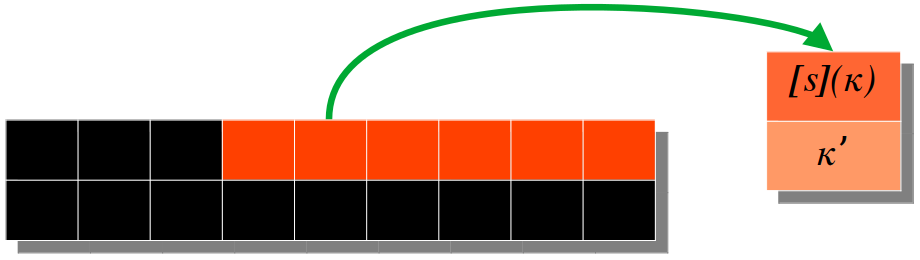
\includegraphics[width=1\textwidth]{conditional}
  \caption{Conditional Analogy}
\label{fig:qafny-con-analog}
\end{minipage}
&
\begin{minipage}[t]{0.3\textwidth}
  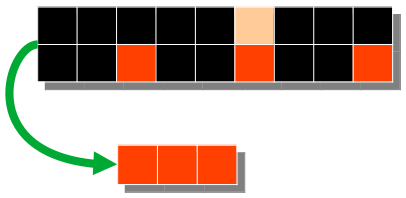
\includegraphics[width=1\textwidth]{measure}
  \caption{Measurement Analogy}
\label{fig:qafny-mea-analog}
\end{minipage}
&
\begin{minipage}[t]{0.3\textwidth}
  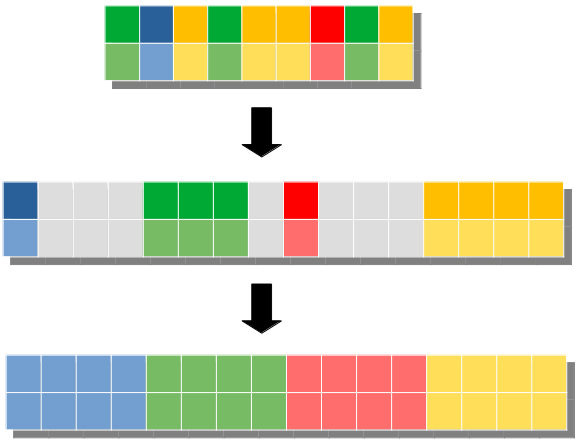
\includegraphics[width=1\textwidth]{diffuse}
  \caption{Diffusion Analogy}
\label{fig:qafny-dis-analog}
\end{minipage}
\end{tabular}
}
\end{figure*}

\myparagraph{Oracle Applications}\label{sec:oracle-state}
The \qafny oracle application $\ssassign{\kappa}{}{\mu}$ is analogized to classical array map operation as discussed in \Cref{fig:intro-example-analog}. Here, assume that $\mu$ works on session $\kappa\uplus \kappa'$. For each element $z_j\ket{c_{j}}{\beta_j}$ in the $\tcht$ type state, we first find $c_{j}$ as the corresponding basis state bitstring for the $\kappa$ session fragment \footnote{ $\kappa$ and $c_{j}$ have the same length and are the prefix session and basis state, respectively.}, then we apply $\mu$ only on $c_{j}$, which is described in the semantic rule \textsc{SA-CH}. Rule \textsc{PA-CH} describes the proof rule for capturing the array map analogy, which has the exact behavior as the semantic rule.
%For example, in the loop body in \Cref{fig:shorqafny} line 11, we apply $\ssassign{y}{}{a^{2^j}y\;\%\; N}$ to a state $y[0..n] \mapsto \schai{2^{j}}{\frac{1}{\sqrt{2^{j}}}}{\tos{a^{\tos{i}}\;\%\;N}}{\ket{\tos{i}.1}}$  \footnote{The state is inside a quantum conditional so the $x[0..j]$ part is masked, and the original one is $\{x[0..j],y[0..n]\} \mapsto \schai{2^{j}}{\frac{1}{\sqrt{2^{j}}}}{\tos{i}.0}{\ket{a^{\tos{i}}\;\%\;N}}+ \schai{2^{j}}{\frac{1}{\sqrt{2^{j}}}}{\tos{i}.1}{\ket{a^{\tos{i}}\;\%\;N}}$ and $\tos{i}$ has $j$ bits. }.  The result is $\schai{2^{j}}{\frac{1}{\sqrt{2^{j}}}}{\tos{a^{\tos{j}.1}\;\%\;N}}{\ket{\tos{i}.1}}$  \footnote{We take the bitstring exponent formula as: $a^{c}= a^{\sum_{j}^{2^{c[j]}}}$, where $c[j]$ is the $j$-th position of $c$. }.
The other similar rules, such as state preparation rules, can be found in \Cref{sec:qafny-app}. 

\begin{figure*}[t]
{\footnotesize
  \begin{mathpar}
    \inferrule[]{R \\ \Omega;\sigma;\varphi\models \kappa \mapsto \scha{m}{z_j}{\beta_j}{\ket{c_j}}}
          {\Omega;\sigma;\varphi\models \mathpzc{M}(b,\kappa) 
              \mapsto \scha{m}{z_j}{c_{j}}{\ket{\beta_j}}+q(\kappa,\neg b) }

    \inferrule[]{R
            \\\Omega;\sigma,\varphi\models \kappa \mapsto \scha{m'}{z'_j}{c_{j1}.c'_{j2}\,\beta_j}+q(\kappa,\neg b)}
          {\Omega;\sigma,\varphi\models \mathpzc{U}(\neg b,\kappa) \mapsto \scha{m}{z_j}{c_{j1}}{\ket{c_{j2}}\ket{\beta_j}}+q(\kappa,\neg b)
  \\\\ \\ * \mathpzc{U}(b,\kappa) \mapsto \scha{m'}{z'_j}{c'_{j2}}{\ket{\beta_j}\ket{c_{j1}}} }

\inferrule[SIF]{ R \\ FV(\emptyset,s)\subseteq \kappa'
          \\(\psi,\varphi[\kappa'\mapsto \scha{m}{z_j}{c_{j2}}{\ket{\beta_j}\ket{c_{j1}}}],s) 
      \to (\psi,\varphi[\kappa'\mapsto \scha{m'}{z'_j}{c'_{j2}}{\ket{\beta_j}\ket{c_{j1}}}],s') } 
{(\psi,\varphi[\kappa\uplus\kappa'\mapsto \scha{m}{z_j}{c_{j1}}{\ket{c_{j2}}\ket{\beta_j}}+q(\kappa,\neg b)],\sifq{b}{s}) \to 
          (\psi,\varphi[\kappa\uplus\kappa'\mapsto \scha{m'}{z'_j}{c_{j1}}{\ket{c'_{j2}}\ket{\beta_j}}+q(\kappa,\neg b)],\sifq{b}{s'}) }

    \inferrule[PIF]{\Omega;\{\kappa' : \tcht\} \vdash Q' \\ \fivepule{\Omega}{\sigma[\kappa' \mapsto \tcht]}{\mmode}{P[\mathpzc{M}(b,\kappa')/ \kappa \uplus \kappa']}{s}{Q * Q'}}
                {\fivepule{\Omega}{\sigma[\kappa \uplus \kappa' \mapsto \tcht]}{g}{P}{\sifq{b}{s}}{P[\mathpzc{U}(\neg b,\kappa \uplus \kappa')/\kappa \uplus \kappa')] * Q'[\mathpzc{U}(b,\kappa \uplus \kappa')/\kappa']}}

\mprset{flushleft}
    \inferrule[SLOOP]{ n_1 < n_2 \\ b'=b[n_1/j] \\ s' =s[n_1/j] }
                  {(\psi,\varphi,\sqwhile{j}{n_1}{n_2}{b}{s}) \longrightarrow \\\\ \quad (\psi,\varphi,\sseq{\sifq{b'}{s'}}{\sqwhile{j}{\texttt{S}\;n_1}{n_2}{b}{s})}}

    \inferrule[PLOOP]{n_1 < n_2\\ \fivepule{\Omega}{\sigma}{\mmode}{P(j)\wedge j \,\slt\, n_2}{\sifq{b}{s}}{P(\snext{j})} }
     {\fivepule{\Omega}{\sigma}{g}{P(n_1)}{ \sqwhile{j}{n_1}{n_2}{b}{s} }{P(n_2)} }

  \end{mathpar}
}
{\footnotesize
\[
\begin{array}{l}
q(\kappa,\neg b) = \schai{m}{z_i}{c_{i}}{\beta_i}
\;\;\texttt{where}\;\forall i.\;\slen{c_{i}}=\slen{\kappa}\wedge \denote{\neg b[c_{i}/\kappa]}
\\[0.2em]
R = FV(\emptyset,b)=\kappa \wedge \forall j.\; \slen{c_{j}}=\slen{\kappa}\wedge\denote{b[c_{j}/\kappa]}
\end{array}
\]
}
\caption{Semantic and Proof Rules for Conditionals and For-loops. $\mathpzc{M}$ is the frozen function and $\mathpzc{U}$ is the unfrozen function. $\denote{b[c_{j}/\kappa]}$ is the interpretation of Boolean guard $b$ by replacing qubits mentioned in $\kappa$ with bits in bitstring $c_{j}$.  $P(j)$ is a predicate $P$ with $j$ as a variable. }
\label{fig:qafny-mu-rules}
\end{figure*}



\myparagraph{Rules for Conditionals and For-Loops}\label{sec:conditionals}
\Cref{fig:qafny-con-analog} describes the analogy of quantum conditionals in \qafny, which are partial map functions that only apply applications on the red parts and freeze the black parts.
It contains two levels of freezing. For each basis state in a session $\kappa_b\uplus \kappa_a$, it freezes the $\kappa_b$ part of the state, which is indicated as the marked black items in the second line in \Cref{fig:qafny-con-analog}. For each basis state in $\scha{m}{z_j}{c_{j1}}{\ket{c_{j2}}\ket{\beta_j}}$ with $\slen{c_{j1}} = \slen{\kappa_b}$, we freeze the $c_{j1}$ part by pushing it to the end of the basis state as $z_j\ket{c_{j2}}\ket{\beta_j}\ket{c_{j1}}$, which is indicated in rule \textsc{SIF} (\Cref{fig:qafny-mu-rules}). 
During the process, the state session is changed from $\kappa_b\uplus \kappa_a$ to $\kappa_a$ when we start evaluating the conditional body $s$. It indicates that the $\kappa_b$/$\ket{c_{j1}}$ part is frozen, because the session is shorter, the $\ket{c_{j1}}$ part is stored in a location beyond the reachable of session $\kappa_a$; therefore, in evaluating $s$, no operation can touch the $\ket{c_{j1}}$ part.
The second level of freezing happens in selecting valid basis states by evaluating the Boolean condition $b$ on basis state bitstrings. Predicate $R$ in rule\textsc{SIF} reflects such task.
Here, we divide the state into two parts as $\scha{m}{z_j}{c_{j1}}{\ket{c_{j2}}\ket{\beta_j}}$ and $q(\kappa,\neg b)$, where the first part contains all basis states satisfying $b$: if we replace the qubit variables in $b$ with $c_{j1}$, the evaluation $\denote{b[c_{j1}/\kappa]}$ is true; while the second part $q(\kappa,\neg b)$ contains all basis states that evaluate $b$ to false.
After the freezing step, we execute $s$ only on the selected unfrozen parts of the state, and merge the execution results ($z'_j$ and $c'_{j2}$) back to the whole state.
The result state element number $m'$ might be different from the pre-execution one ($m$) because applications in $s$ might increase the state numbers such as applying a quantum diffusion operation.

To design a proof rule for such partial map, we develop the frozen ($\mathpzc{M}$) and unfrozen ($\mathpzc{U}$) operations with the session types. Both take a Boolean expression $b$ and a quantum state as arguments. As shown on top of \Cref{fig:qafny-mu-rules}, $\mathpzc{M}$'s modeling materializes the freezing mechanism above. For a state $\scha{m}{z_j}{c_{j1}}{\ket{c_{j2}}\ket{\beta_j}}+q(\kappa,\neg b)$, we keep the basis states satisfying $b$, as shown in predicate $R$, remove the unsatisfied basis states $q(\kappa,\neg b)$, and push the basis bitstrings $c_{j1}$ to the state stacks.
In the pre-condition manipulation of rule \textsc{PIF}, we substitute $\kappa \uplus \kappa'$ with $\mathpzc{M}(b,\kappa')$. During the process, the session type in $\sigma$ is changed from $\kappa \uplus \kappa'$ to $\kappa'$.
Function $\mathpzc{U}$ unfreezes the state by assembling the result state of applying $s$ to the frozen $\kappa \uplus \kappa'$ state (the black part in \Cref{fig:qafny-con-analog}). It is always appeared as a pair with both the $b$ and $\neg b$ cases, referring to the two state divisions above. In the post-condition manipulation, we substitute $\kappa \uplus \kappa'$ with $\mathpzc{U}(\neg b,\kappa \uplus \kappa')$ in $P$, representing the unchanged and frozen state; and substitute $\kappa'$ with $\mathpzc{U}(b,\kappa \uplus \kappa')$ in $Q'$, representing the result of applying $s$ on the unfrozen part, and assemble them together through the separation operation $*$. 
$\Omega;\{\kappa' : \tcht\} \vdash Q'$ ensures that $Q'$ only mentions session $\kappa'$.
$\mathpzc{U}$'s modeling in the first line of \Cref{fig:qafny-mu-rules} captures the assemble procedure by merging two $\mathpzc{U}$ constructs together. Rules \textsc{SLOOP} and \textsc{PLOOP} are the semantic and proof rules for a for-loop, which is a simplified version of while-loop in classical separation logic, because for-loop is guaranteed to terminate.

{\footnotesize
  \begin{mathpar}
\mprset{flushleft}
\inferrule[]{
   \inferrule[]
   { \inferrule[] 
{\fivepule{\Omega}{\{\kappa:\tcht\}}{\mmode}
{\textcolor{teal}{
\kappa\mapsto {\frac{1}{\sqrt{2}}}\ket{\overline{1}}\ket{0}}
\textcolor{purple}{
\ket{1}
}
}{ s }{
\textcolor{teal}{
\kappa\mapsto {\frac{1}{\sqrt{2}}}\ket{\overline{1}}\ket{1}}
\textcolor{purple}{
\ket{1}
}
}
 }
  { \fivepule{\Omega}{\{\kappa:\tcht\}}{\mmode}
{\textcolor{teal}{
\mathpzc{M}(x[j],\kappa)\mapsto
  \schii{2}{\frac{1}{\sqrt{2}}}{\overline{i}}\ket{0}
}
}{ s }{
\textcolor{teal}{
\kappa\mapsto {\frac{1}{\sqrt{2}}}\ket{\overline{1}}\ket{1}}
\textcolor{purple}{
\ket{1}
}
}
} }
   {
\fivepule{\Omega}{\{\kappa_1:\tcht\}}{\cmode}
{\textcolor{teal}{
\kappa_1\mapsto \schii{2}{\frac{1}{\sqrt{2}}}{\overline{i}}\ket{0}
}
}{ \sifq{x[j]}{s} }{
\textcolor{teal}{
\mathpzc{U}(\neg x[j],\kappa_1)\mapsto \schii{2}{\frac{1}{\sqrt{2}}}{\overline{i}}\ket{0}
*
\mathpzc{U}(x[j],\kappa_1)\mapsto {\frac{1}{\sqrt{2}}}\ket{\overline{1}}\ket{1}
}
\textcolor{purple}{
\ket{1}
}
}} } {
\fivepule{\Omega}{\sigma}{\cmode}
{\textcolor{teal}{
x[0..\snext{j}]\mapsto \schii{2}{\frac{1}{\sqrt{2}}}{\overline{i}} * x[\snext{j}..n]\mapsto \ket{\overline{0}}
}
}{ \sifq{x[j]}{s} }{
\textcolor{teal}{
x[0..j\splus\,2]\mapsto \schii{2}{\frac{1}{\sqrt{2}}}{\overline{i}} * x[j\,\splus\,2..n]\mapsto \ket{\overline{0}}
} } }
  \end{mathpar}
{
\begin{center}
$\begin{array}{l}
\kappa=\{x[0..j],x[\snext{j}..j\,\splus\,2]\}
\quad
\kappa_1=\{x[j..\snext{j}\} \uplus \kappa
\quad
s=\ssassign{x[\snext{j}]}{}{x[\snext{j}]+1};
\quad
\sigma=\{x[0..\snext{j}]: \tcht, x[\snext{j}..n]: \tnort\}
\end{array}$
\end{center}
}
}

As an example, we show the proof, built from bottom up, for a GHZ loop-step above.
We first move a $\tnort$ type qubit $x[\snext{j}]$ to session $x[0..\snext{j}]$ and use the \rulelab{Frame} rule to disregard session $x[j\,\splus\,2..n]$. We then apply rule \rulelab{PIF} to freeze the qubit $x[j]$, with the basis state having $x[j]=0$ disregarded, and left with the state $\textcolor{teal}{{\frac{1}{\sqrt{2}}}\ket{\overline{1}}\ket{0}}\textcolor{purple}{\ket{1}}$, with the purple part also being frozen.
Notice that $\kappa_1$ has the same qubits as session $x[0..j\splus\,2]$ 
with different arrangement by applying some equivalence state rewrites.
We apply rule \textsc{PA-CH} at the top and flip the $0$ bit. As the post-condition of rule \rulelab{PIF}, we use two $\mathpzc{U}$ functions to assemble the state $\textcolor{teal}{{\frac{1}{\sqrt{2}}}\ket{\overline{1}}\ket{1}}\textcolor{purple}{\ket{1}}$ back to the state of session $\kappa_1$.

\begin{figure*}[t]
{\footnotesize
  \begin{mathpar}

    \inferrule[]{\slen{c}=n \\
           \Omega;\sigma;\varphi\models \kappa \mapsto 
                      \sch{m}{\frac{z_j}{\sqrt{r}}}{c_{j}} \wedge x = (r,\tov{c})}
          {\Omega;\sigma,\varphi\models \mathpzc{F}(x,n,\kappa) \mapsto \scha{m}{z_j}{c}{\ket{c_{j}}}+q(n,\neq c) }

\mprset{flushleft}
    \inferrule[SMea]{\varphi(y) = \{y[0..n]\uplus\kappa\mapsto \scha{m}{z_j}{c}{\ket{c_{j}}}+q(n,\neq c)\}}{(\psi,\varphi,\sexp{x}{\smea{y}}{s}) \longrightarrow \\\\\quad (\psi[x\mapsto (r,\tov{c})],\varphi[\kappa \mapsto  \sch{m}{\frac{z_j}{\sqrt{r}}}{c_{j}}],s) }

    \inferrule[PMea]{\fivepule{\Omega[x\mapsto \mmode]}{\sigma[\kappa\mapsto \tcht]}{\cmode}{P[\mathpzc{F}(x,n,\kappa)/y[0,n]\uplus\kappa]}{s }{Q} }
     {\fivepule{\Omega[y\mapsto \qmode{n}]}{\sigma[y[0,n]\uplus\kappa\mapsto \tcht]}{\cmode}{P}{\sexp{x}{\smea{y}}{s} }{Q} }

  \end{mathpar}
}
{\footnotesize
\[r= \sum_{k=0}^{m} \slen{z_k}^2
\qquad\qquad
q(n,\neq c) = \schk{m'}{z'_k}{c'.c'_{k}} \;\;\texttt{where}\;c'\neq c\]
}
\caption{Semantic and Proof Rules for Measurement. $\mathpzc{F}$ is the measurement function construct. $\tov{c}$ turns bitstring $c$ to an integer, and $r$ is the likelihood that the bitstring $c$ appears in a basis state. }
\label{fig:qafny-mea-rules}
\end{figure*}

\myparagraph{Measurement Rules}\label{sec:measurement}
%
As \Cref{fig:qafny-mea-analog} describes, quantum measurement is a two-step array filter: 1) The session is partitioned into two parts, so do all the basis states, and we randomly pick a basis state first part as a key (the pink part); and 2) we create a new array by cutting all elements' first parts with keeping the elements whose original first part is equal to the key.
Notice that the the red basis states appear in a periodical pattern in the whole array. This behavior is universally true for quantum operations, and many quantum algorithms utilize the periodical pattern.

In rule \textsc{SMea} in \Cref{fig:qafny-mea-rules}, we pick an $n$-length bitstring $c$ as the pink key and collect $m$ basis states $\scha{m}{z_j}{c}{\ket{c_{j}}}$ that has the key $c$. In the post-state, we update the remaining session $\kappa$ to $\sch{m}{\frac{z_j}{\sqrt{r}}}{c_{j}}$ with the adjustment of amplitude $\frac{1}{\sqrt{r}}$, and replace the variable $x$ in the statement $s$ with the value $(r,\tov{c})$.
In designing the proof rule \textsc{PMea}, a session type operation $\mathpzc{F}(x,n,\kappa)$ is invented to do exactly the two steps above by selecting an $n$-length prefix bitstring $c$ in a basis state for range $y[0..n]$, computing the probability $r$, and assigning $(r,\tov{c})$ to variable $x$.
Rule \textsc{PMea} replaces session $y[0..n]\cup \kappa$ in $P$ with the measurement result session $\mathpzc{F}(x,n,\kappa)$ and updates the type state $\Omega$ and $\sigma$ by replacing $y[0..n]\cup \kappa$ with $\kappa$. 

{\footnotesize
  \begin{mathpar}
   \inferrule[]
   { \fivepule{\Omega[u\mapsto \mmode]}{\{x[0..n] : \tcht\}}{\cmode}
  {\textcolor{teal}{\mathpzc{F}(u,n,x[0..n])\mapsto C}}{ \{\} }{\textcolor{teal}{x[0..n] \mapsto D * E}} }
   { \fivepule{\Omega}{\{\{y[0..n],x[0..n]\} : \tcht\}}{\cmode}
      {\textcolor{teal}{\{y[0..n],x[0..n]\}\mapsto C}}{ \sexp{u}{\smea{y}}{\{\}} }{\textcolor{teal}{x[0..n] \mapsto D * E}}
     }
  \end{mathpar}
{
\begin{center}
$\begin{array}{l}
C \triangleq \sch{2^{n}}{\frac{1}{\sqrt{2^{n}}}}{\tos{a^{j}\;\%\;N}.\tos{j}}
\quad
D \triangleq \smch{\frac{1}{\sqrt{s}}}{s}{t\,\splus\,k p}
\quad
E \triangleq p = \texttt{ord}(a,N)
\wedge
u=(\frac{s}{2^n},a^{t}\;\%\;N)
\wedge
s=\texttt{rnd}(\frac{2^n}{p})
\end{array}$
\end{center}
}
}

Here, we show a proof fragment above for the partial measurement in line 14 in \Cref{fig:shorqafny}.
The proof applies rule $\textsc{PMea}$ by replacing session $\{x[0..n],y[0..n]\}$ with $\mathpzc{F}(u,n,x[0..n])$.
On the top, the pre- and post-conditions are equivalent as explained below.
In session $\{y[0..n],x[0..n]\}$, range $y[0..n]$ stores the basis state $\tos{a^{j}\;\%\;N}$, which contains value $j$ that represents the basis states for group $x[0..n]$. Selecting a basis state $a^{t}\;\%\;N$ also filters the $j$ in $x[0..n]$, such that we pick any $j$ having the relation $a^{j}\;\%\;N=a^{t}\;\%\;N$. Notice that modulo multiplication is a periodical function, which means that the relation can be rewritten $a^{t+kp}\;\%\;N=a^{t}\;\%\;N$, such that $p$ is the order. Thus, the $x[0..n]$ state is rewritten as a summation of $k$: $\smch{\frac{1}{\sqrt{s}}}{s}{t\,\splus\,k p}$. The probability of selecting $\tos{a^{j}\;\%\;N}$ is $\frac{s}{2^n}$.
In \qafny, we set up additional axioms for these periodical theorems to grant this kind of pre- and post-condition equivalence.

\begin{figure*}[t]
{\small
  \begin{mathpar}

    \inferrule[SDis]{FV(\Omega,l)=\kappa \\ \varphi(\kappa) = \{\kappa\uplus\kappa'\mapsto q\}}
      {(\varphi,\ssassign{l}{}{\sdis}) \longrightarrow (\varphi[\kappa\uplus\kappa' \mapsto \mathpzc{D}(\slen{\kappa},q)],\{\}) }

    \inferrule[PDis]{ FV(\Omega,l)=\kappa\\\sigma(\kappa)=\{\kappa\uplus\kappa:\tcht\} }
     {\fivepule{\Omega}{\sigma}{g}{\kappa\uplus\kappa'\mapsto q}{\ssassign{l}{}{\sdis} }{\kappa\uplus\kappa'\mapsto \mathpzc{D}(\slen{\kappa},q)} }
  \end{mathpar}
}
{\footnotesize
$
\mathpzc{D}(n,\Msum_{i=0}^{m}\scha{2^{n}}{z_{ij}}{j}{\ket{c_{ij}}})=\Msum_{i=0}^{m}\scha{2^n}{(\frac{1}{2^{n-1}}\sum_{u=0}^{2^n}z_{iu} - z_{ij})}{j}{\ket{c_{ij}}}
$
}
\caption{Semantic and Proof Rules for Diffusion Operations}
\label{fig:exp-proofsystem-5}
\end{figure*}

\myparagraph{Rules for Diffusion}\label{sec:diffuse}
Quantum diffusion operations ($\ssassign{l}{}{\sdis}$) reorient the amplitudes of basis states based on the basis state corresponding to $l$. They are analogized to an aggregate operation of reshape and mean computation, both appeared in some programming languages, such as Python.
The aggregate operation first applies a reshape, where elements are regrouped into a normal form, as the first arrow of \Cref{fig:qafny-dis-analog}. More specifically, the diffusion function $\mathpzc{D}(n,q)$ (\Cref{fig:exp-proofsystem-5}) first takes an $n'$-element $\tcht$ type state $\schi{t=0}{z_t}{c_t}$, where $n$ corresponds to the number of qubits in $l$.
Then, we rearrange the state by extending the element number from $n'$ to $m*n$ with probably adding new elements that originally have zero amplitude (the white elements in \Cref{fig:qafny-dis-analog}).
Here, let's view a basis $c_{t}$ as a small-endian (LSB) number $\tov{c_{t}}$. The rearrangement of changing bases $c_{t}$ (for all $t$) to $\tos{j}.c_{ij}$ is analogized to rewrite a number $\tov{c_{t}}$ to be the form $2^n i+j$, with $j\in [0,2^n)$,
i.e., the reshape step rearranges the basis states to be a periodical counting sequence, with $2^n$ being the order.
The mean computation analogy (the second arrow in \Cref{fig:qafny-dis-analog}) takes every period in the reshaped state, and for each basis state in a period, we redistribute its amplitude by the formula $(\frac{1}{2^{n-1}}\sum_{u=0}^{2^n}z_{iu} - z_{ij})$.
Rule \textsc{SDis} is the semantics for diffusion $\ssassign{l}{}{\sdis}$, which applies the $\mathpzc{D}$ function to session $\kappa \uplus \kappa'$, where $\kappa$ contains all qubits in $l$. Proof rule \textsc{PDis} is a separation style rule that does the same as rule \textsc{SDis}.
\ignore{
Quantum diffusion operations are used in many algorithms, such as amplifying a basis state's amplitude value in Grover's search algorithm, or redistributing a possible path direction in quantum walk algorithm.
In these algorithms, the session piece that is diffused has either a small constant number of qubits or the whole session, meaning that the $n$ number in the $\mathpzc{D}$ function is either very small or equal to $\slen{\kappa \uplus \kappa'}$, as the whole session.
In either case, the summation formula in $\mathpzc{D}$'s modeling (\Cref{fig:qafny-dis-model}) can be rewritten as very few terms that facilitate the automated verification, which is exactly how we handle the diffusion operations in \qafny.
}
An example of quantum walk algorithm that uses diffusion operations is given in \Cref{sec:quantumwalk}.

\subsection{\qafny Metatheory}\label{sec:theorems}

Here, we show the type soundness and proof system soundness and completeness.

\myparagraph{Type Soundness}
We prove that well-typed \qafny programs are well defined; i.e., the
type system is sound with respect to the semantics, with the well-formedness assumptions (\Cref{def:well-formed-ses} and \Cref{def:well-formed}).
The \qafny type soundness is stated as two theorems, type progress and preservation . The proofs are done by induction on statements $s$ and mechanized in Coq.

\begin{theorem}[\qafny type progress]\label{thm:type-progress-oqasm}\rm 
If $\Omega;\sigma \vdash_g s \triangleright \sigma'$ and $\Omega;\sigma \vdash \varphi$, then either $s=\{\}$, or there exists $\varphi'$ and $s'$ such that $(\varphi,s)\longrightarrow (\varphi',s')$.
\end{theorem}

\begin{theorem}[\qafny type preservation]\label{thm:type-preservation-oqasm}\rm 
If $\Omega;\sigma \vdash_g s \triangleright \sigma'$, $\Omega;\sigma \vdash \varphi$, and $(\varphi,s)\longrightarrow (\varphi',s')$, then 
there exists $\Omega'$ and $\sigma''$, $\Omega';\sigma'' \vdash_g s' \triangleright \sigma'$ and $\Omega';\sigma'' \vdash \varphi'$.
\end{theorem}

\myparagraph{Proof System Soundness and Completeness}
We prove that the \qafny proof system is sound and complete with respect to it semantics for well-typed \qafny programs.
In \qafny, there are three different state representations for a session $\kappa$ and two sessions can be joined into a large session.
Hence, given a statement $s$ and an initial state $\psi$ and $\varphi$, the semantic transition $(\psi, \varphi,s) \longrightarrow^{*} (\psi',\varphi',\{\})$ might not be unique, such that there might be different $\varphi'$ representations.
However, any $\tnort$ and $\thadt$ type state can be represented as a $\tcht$ type state, so that $\tcht$ type states can be viewed as the \emph{most general} state representation. We also have state equivalence relations defined for capturing the behaviors of session permutation, join and split. We define the \emph{most general state representation} of evaluating a statement $s$ in an initial state $\varphi$ below.

\begin{definition}[Most general \qafny state]\label{def:most-gen}\rm 
  Given $s$, $\varphi$, $\Omega$, $\sigma$, and $g$, such that $\Omega;\sigma\vdash_g \varphi$, $\Omega;\sigma\vdash_g s \triangleright \sigma^*$, $\Omega;\sigma[\uparrow \sigma^*]\vdash \varphi^*$, and $(\psi,\varphi,s) \longrightarrow^{*} (\psi',\varphi^*,\{\})$, $\varphi^*$ is the most general state representation of evaluating $(\psi,\varphi,s)$, iff for all $\sigma'$ and $\varphi'$, such that $\Omega;\sigma\vdash_g s \triangleright \sigma'$, $\Omega;\sigma[\uparrow \sigma']\vdash \varphi'$ and $(\psi,\varphi,s) \longrightarrow^{*} (\psi',\varphi',\{\})$, $\sigma' \preceq \sigma^*$ and $\varphi' \equiv \varphi^*$.
\end{definition}

The \qafny proof system correctness is defined by the soundness and relatively completeness theorems below, which has been formalized and proved in Coq. The \qafny proof system only describes the quantum portion built on top of the Dafny system. Since the quantum portion contains non-terminated programs, the soundness and completeness essentially refers to the partial correctness of the \qafny proof system and the total correctness is achieved by compiling \qafny programs to Dafny. The \qafny proof system correctness is defined in terms of programs being well-typed. The type soundness theorem suggests that any intermediate transitions of evaluating a well-typed \qafny program is also well-typed. Thus, the proof system correctness proof only reason about well-typed predicates in \Cref{def:well-formed}.


\begin{theorem}[proof system soundness]\label{thm:proof-soundness}\rm 
For a well-typed program $s$, such that $\Omega;\sigma\vdash_g s \triangleright \sigma'$, $\fivepule{\Omega}{\sigma}{g}{P}{s}{Q}$, $\Omega;\sigma;\psi;\varphi\models_g P$, then there exists a state representation $\varphi'$, such that $(\psi,\varphi,s)\longrightarrow^* (\psi',\varphi',\{\})$ and $\Omega;\sigma[\uparrow\sigma'];\psi';\varphi'\models_g Q$, and there is a most general state representation $\varphi^*$ of evaluating $(\psi,\varphi,s)$ as $(\psi,\varphi,s)\longrightarrow^* (\psi',\varphi^*,\{\})$ and $\varphi' \equiv \varphi*$.
\end{theorem}

\begin{theorem}[proof system relative completeness]\label{thm:proof-completeness}\rm 
For a well-typed program $s$, such that $\Omega;\sigma\vdash_g s \triangleright \sigma'$, $(\psi,\varphi,s)\longrightarrow^* (\psi',\varphi',\{\})$ and $\Omega;\sigma\vdash_g \varphi$, there is most general state representation $\varphi^*$, such that $(\psi,\varphi,s)\longrightarrow^* (\psi',\varphi',\{\})$ and $\varphi' \equiv \varphi^*$ and $\Omega;\sigma\vdash_g s \triangleright \sigma^*$ and $\Omega;\sigma[\uparrow \sigma^*]\vdash_g \varphi^*$, and there are predicates $P$ and $Q$, such that $\Omega;\sigma;\psi;\varphi\models_g P$ and $\Omega;\sigma[\uparrow\sigma^*];\psi';\varphi^* \models Q$ and $\fivepule{\Omega}{\sigma}{g}{P}{s}{Q}$.
\end{theorem}




